\documentclass[a4paper,12pt]{article}

%Eingabe deutscher Umlaute
\usepackage[utf8]{inputenc}
\usepackage[T1]{fontenc}
\usepackage[ngerman]{babel}

\usepackage[colorlinks=true,linkcolor=green]{hyperref}


%Mathematische Symbole
\usepackage{amsmath}
\usepackage{mathtools}
\usepackage{amsthm}
\newtheorem{theorem}{Theorem}
\usepackage{amssymb}
\usepackage{mathdots}
\usepackage{bbm}
\usepackage{textgreek}
\usepackage[linewidth=1pt]{mdframed}
\usepackage{blindtext}

\usepackage[pdftex]{graphicx}

 %Weniger breite Raender
 \usepackage{a4wide}
\usepackage[right = 2cm, top=2cm, bottom=2.5cm,left=2cm]{geometry} 


%Normale Papiereinstellungen; Kein Einzug bei neuem Absatz.
\pagestyle{plain}
\setlength\parindent{0pt}


%%%%%%%%%%%%%%%%%%%%%%%%%%
%%%%%%%%Abkuerzende Befehle%%%%%%%
%%%%%%%%%%%%%%%%%%%%%%%%%%
%Erstes Argument {} enthaelt jeweils die Abkuerzung, zweites Argument {} den Latex-Befehl

% Zahlbereiche
\newcommand{\IN}{\mathbb{N}}
\newcommand{\IQ}{\mathbb{Q}}
\newcommand{\IZ}{\mathbb{Z}}
\newcommand{\IR}{\mathbb{R}}
\newcommand{\IC}{\mathbb{C}}

%Wahrscheinlichkeit und Erwartungswert
\newcommand{\IP}{\mathbb{P}}
\newcommand{\IE}{\mathbb{E}}

%Indikatorfunktion
\newcommand{\Ii}{\mathbbm{1}}

%Abkuerzungen fuer Sigma-Algebren etc.
\newcommand{\sP}{\mathcal{P}}
\newcommand{\sA}{\mathcal{A}}
\newcommand{\sC}{\mathcal{C}}
\newcommand{\sX}{\mathcal{X}}
\newcommand{\sE}{\mathcal{E}}
\newcommand{\sU}{\mathcal{U}}
\newcommand{\sN}{\mathcal{N}}
\newcommand{\sB}{\mathcal{B}_{\IR}}

\newcommand{\seqA}{$(A_{i})_{i\in\IN}\,$}
\newcommand{\unionA}{$\cup_{i\in\IN}{A_{i}}\,$}

\newcommand{\sig}{\textsigma\,}
\newcommand{\omeg}{\textOmega\,}

\newcommand\defeq{\stackrel{\mathclap{\normalfont\mbox{def}}}{=}}
\newcommand\totprobeq{\stackrel{\mathclap{\normalfont\mbox{LoTP}}}{=}}
\newcommand\propaeq{\stackrel{\mathclap{\normalfont\mbox{(a)}}}{=}}
\newcommand\propbeq{\stackrel{\mathclap{\normalfont\mbox{(b)}}}{=}}

\newcommand{\expKX}{\IE(e^{kX})}
\newcommand{\expKY}{\IE(e^{kY})}
\newcommand{\expX}{\IE(X)}
\newcommand{\gammaF}{\frac{\lambda^{\alpha}}{\Gamma(\alpha)}}
\newcommand{\gammaDenom}{\frac{1}{\Gamma(\alpha)}}
\newcommand{\datFrac}{\left( \frac{1}{\lambda - k} \right)^{\alpha}}
\newcommand{\datFracL}{\left( \frac{\lambda}{\lambda - k} \right)^{\alpha}}
\newcommand{\kdermx}{\frac{dM_{X}}{dk}\big|_{k=0}}
\newcommand{\expint}[1]{\int_{0}^{\infty}{e^{#1 }dx}}

\makeatletter
\renewcommand*{\eqref}[1]{%
  \hyperref[{#1}]{\textup{\tagform@{\ref*{#1}}}}%
}
\makeatother

%Aufzaehlungen bei enumerate werden (a),(b),(c)
\renewcommand{\labelenumi}{(\alph{enumi})}

\title{
	Exercise 7  \\
	\large Computational Statistics and Data Analysis \\
	\large Summer Semester, 2020
	}
\author{Ryan Hutchins \\ 
Ruprecht Karls Universit\"at Heidelberg}
\date{8 Mai, 2020}

\begin{document}
\maketitle

You may find the code for this assignment \href{https://github.com/GoliathMarks/Computational_Statistics/blob/master/CompStatsHomeworkSeven/CompStatsHomeworkSeven.py}{here}.

\section{Problem 1: Numerical Optimization}
\begin{enumerate}
\item MSE = 5.920153095813081
 \begin{figure}[h!]
 \centering
  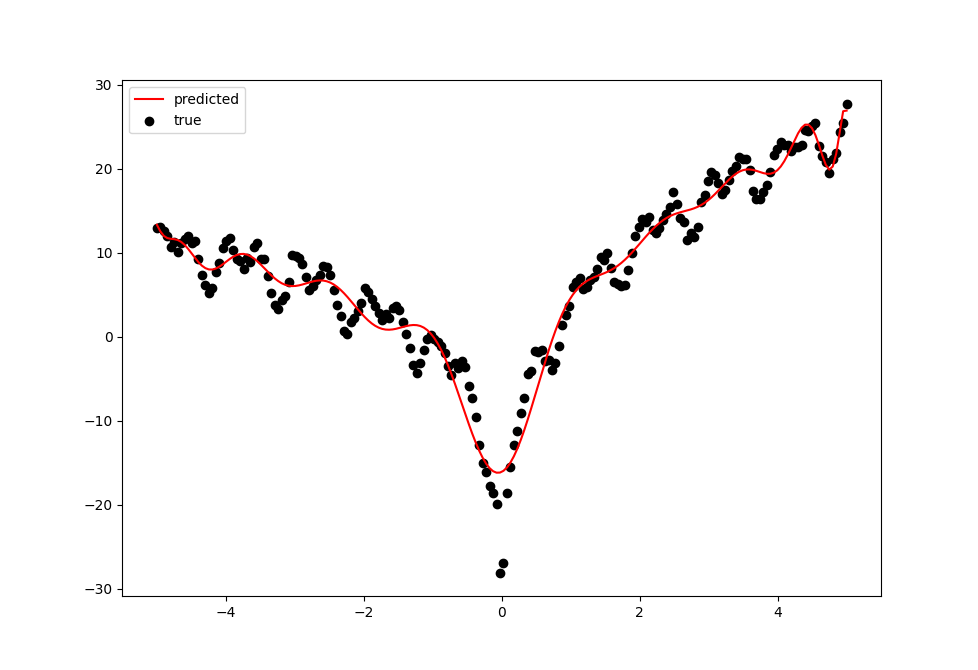
\includegraphics[width=0.5\textwidth]{/home/ryan/PycharmProjects/ComputationalStatistics/WrittenAssignments/images/basis_expansion.png}
 \caption{Graph for part (a)}
 \end{figure}
 
 
\item MSE = 2495.3320839207304
 \begin{figure}[h!]
 \centering
  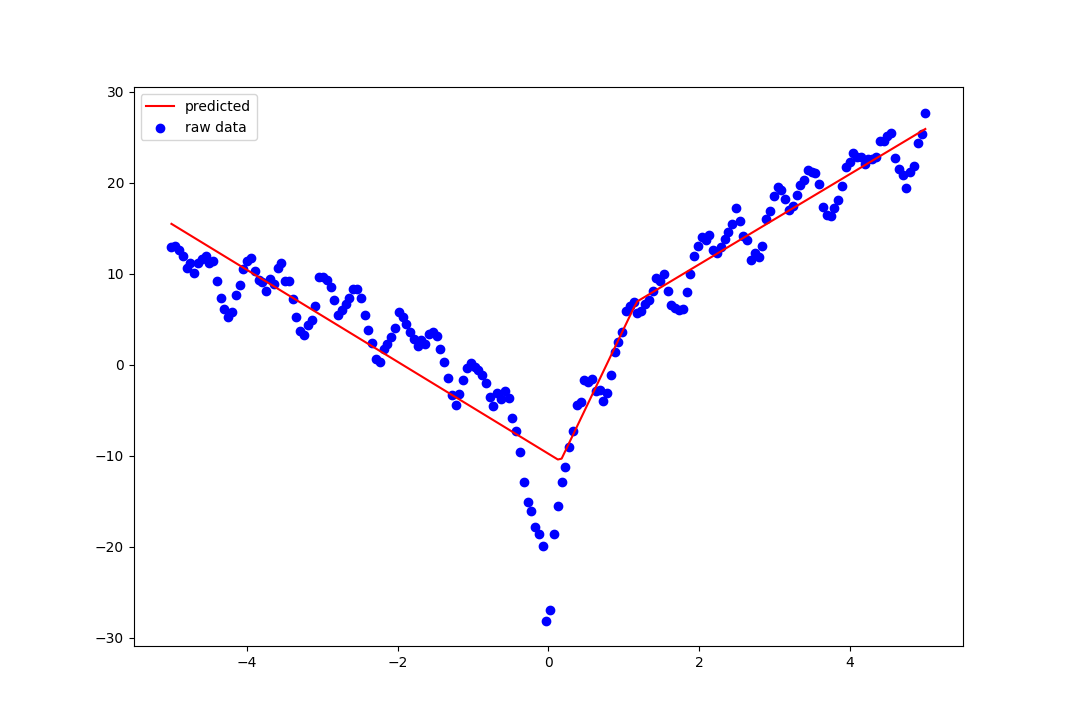
\includegraphics[width=0.5\textwidth]{/home/ryan/PycharmProjects/ComputationalStatistics/WrittenAssignments/images/ANN_1_layer.png}
 \caption{Graph for part (b), 1 layer, 7 units}
 \end{figure}


\item MSE = 3568.3240332006994
 \begin{figure}[h!]
 \centering
  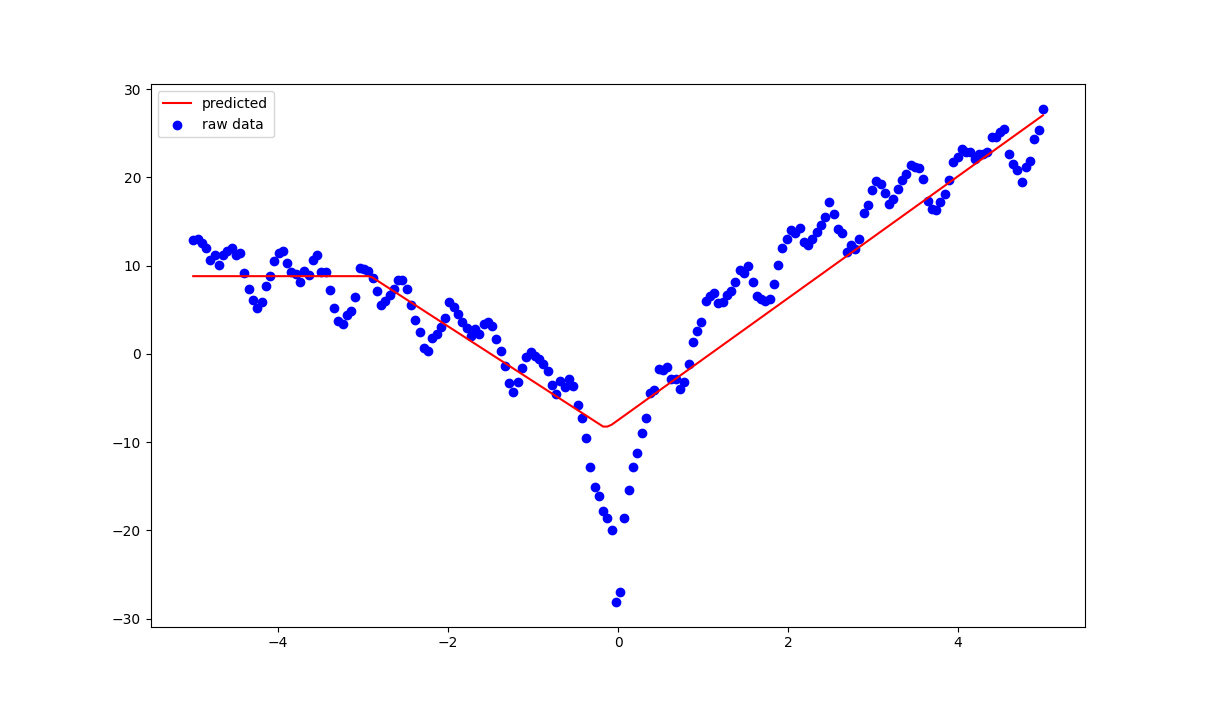
\includegraphics[width=0.5\textwidth]{/home/ryan/PycharmProjects/ComputationalStatistics/WrittenAssignments/images/ANN_2_layer.png}
 \caption{Graph for part (c), 2-layer ANN with 3 units per layer}
 \end{figure}


\item MSE = 1108.147105495679
\begin{figure}[h!]
 \centering
  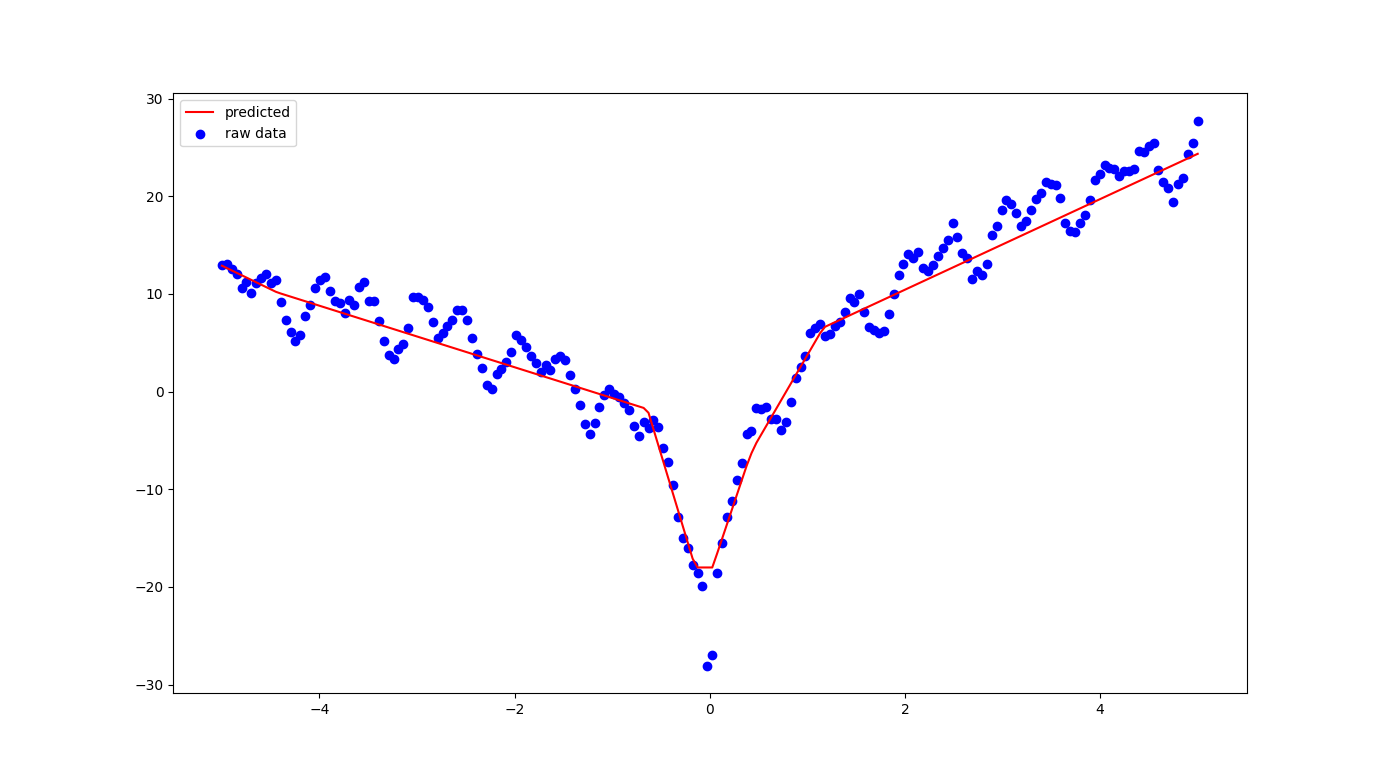
\includegraphics[width=0.5\textwidth]{/home/ryan/PycharmProjects/ComputationalStatistics/WrittenAssignments/images/ANN_2_layer_7_units.png}
 \caption{Graph for part (d), 2-layer ANN with 7 units per layer}
 \end{figure}


\item Using a sigmoid function with two hidden layers, 3 units per layer, made it worse than when I used the leaky rectified linear unit.
\begin{figure}[h!]
 \centering
  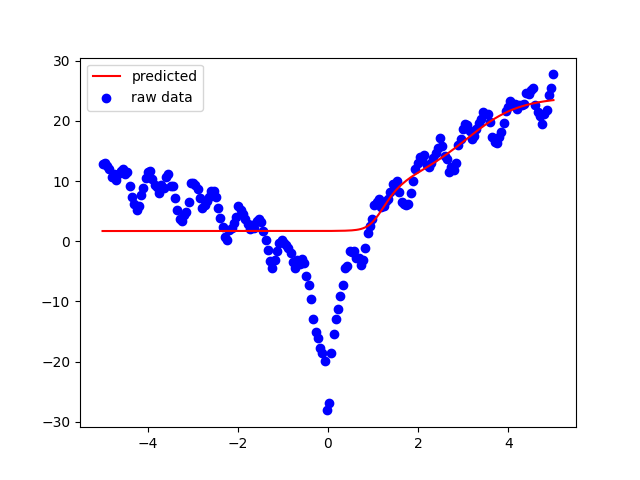
\includegraphics[width=0.5\textwidth]{/home/ryan/PycharmProjects/ComputationalStatistics/WrittenAssignments/images/ANN_2_layer_sigmoid.png}
 \caption{Graph for part (d), 2-layer ANN with 7 units per layer}
 \end{figure}

See next page for additional graphs.
\end{enumerate}






\end{document}